%%%% IACR Transactions TEMPLATE %%%%
% This file shows how to use the iacrtrans class to write a paper.
% Written by Gaetan Leurent gaetan.leurent@inria.fr (2020)
% Public Domain (CC0)


%%%% 1. DOCUMENTCLASS %%%%
\documentclass[journal=tosc,preprint]{iacrtrans}
%%%% NOTES:
% - Change "journal=tosc" to "journal=tches" if needed
% - Change "submission" to "final" for final version
% - Add "spthm" for LNCS-like theorems

% \usepackage[
% backend=biber,
% style=alphabetic,
% sorting=ynt
% ]{biblatex}

%%%% 2. PACKAGES %%%%
% \usepackage{cite}
\usepackage{algorithmic}
\usepackage{textcomp}
\usepackage{xcolor}
\usepackage{mathtools}

\usepackage{amssymb}
% Language setting
% Replace `english' with e.g. `spanish' to change the document language
\usepackage{times,amsmath,amsthm,amsfonts,eucal,graphicx,listings,booktabs,lipsum,multicol} % Example package -- can be removed

\usepackage[colorlinks=true, allcolors=blue]{hyperref}
\usepackage{enumitem}
\usepackage[T1]{fontenc}
\usepackage{babel}
\usepackage[utf8]{inputenc}
%%%% 3. AUTHOR, INSTITUTE %%%%
\author{Manohar Lal Das \and Aman Khan \and Aayush Deshmukh}
\institute{
  IIT Bhilai, Raipur, India, \email{manoharlal@iitbhilai.ac.in}
  \and
  IIT Bhilai, Raipur, India, \email{amankhan@iitbhilai.ac.in}
  \and
  IIT Bhilai, Raipur, India, \email{aayushd@iitbhilai.ac.in}
}
%%%% NOTES:
% - We need a city name for indexation purpose, even if it is redundant
%   (eg: University of Atlantis, Atlantis, Atlantis)
% - \inst{} can be omitted if there is a single institute,
%   or exactly one institute per author


%%%% 4. TITLE %%%%
\title{PRINT Cipher}
%%%% NOTES:
% - If the title is too long, or includes special macro, please
%   provide a "running title" as optional argument: \title[Short]{Long}
% - You can provide an optional subtitle with \subtitle.

\begin{document}

\maketitle


%%%% 5. KEYWORDS %%%%
\keywords{SPN \and IC-printing}


%%%% 6. ABSTRACT %%%%
\begin{abstract}
  Print Cipher is one of the lightweight SPN network with 48-bit and 96-bit block cipher for IC-printing. It is design to make use of the properties of IC-printing technology. Print cipher is still in the beginning phase of their development but allow the production of different circuits at low cost.
\end{abstract}


%%%% 7. PAPER CONTENT %%%%
\section{Introduction}

In order to spot items using smart bar-codes, we use RFID tags and sensors, the safety of contrived hardware devices like RFID tags is a major concern in cryptography nowadays. PRINT Cipher, which was introduced in two forms a 48-bit and another 96-bit cipher, was published in “Cryptographic Hardware and Embedded systems ( CHES 2010 )”. This cipher can have either 80 or 160 bit unrevealed keys. The essential and appealing properties of PRINTcipher are that each one round uses the identical round key and differs only by a round counter in which the linear layer is partially key-dependent. Invariance subspace attacks are promising attack results on PRINT Cipher on the whole Printcipher- 48/96. Here the supported weak keys are considered as the very well known Cryptanalytic result, and the simplest attack encountered is invariance subspace attacks on the complete PRINTcipher - 48/96.
It requires 5 choosen plaintexts that are applicable to PRINT Cipher- 48 attacks which has 2\textsuperscript{53} weak keys, and whose computational complexity is negligible. Similarly 2\textsuperscript{102} Weak Key is there in PRINT Cipher- 96 and the attack requires five chosen plaintexts whose computational complexity is negligible.

\begin{figure}[h]
	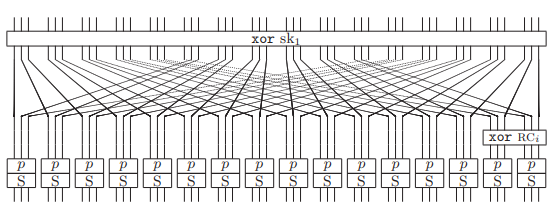
\includegraphics[width=\linewidth]{pics/printcipher.png}
\end{figure}


\section{Main Result}
\label{sec:main}

\subsection{Sbox Analysis}

The sbox for the PRINT cipher is a 3-bit to 3-bit. Since input is 3-bit so for a b-bit block, the sbox is applied $\frac{b}{3}$ parallely. The current state for the sbox is a $\frac{b}{3}$ words, for each word same sbox is used and concatinating the output gives the next state.It is a balanced sbox and has a linear structure.The sbox is shown below :- 

\begin{figure}[ht]
	\centering
	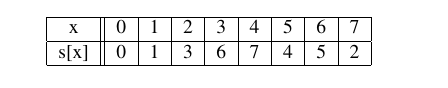
\includegraphics{pics/sbox1.png}
\end{figure}

\subsubsection{Difference Distribution Table}
The sbox has a differential branch number defined as min\textsubscript{v, w $\neq$v} \{wt(v $\oplus$ w) + wt(S(v) $\oplus$ S(w))\} of \textbf{2}. The difference distribution table (ddt) which is generated using Sage is as follows :- 
\begin{table}[h]
	\centering
	\resizebox{7cm}{!}{%
		\begin{tabular}{@{}|l|llllllll|@{}}
			\toprule
			& \multicolumn{1}{c}{0} & \multicolumn{1}{c}{1} & \multicolumn{1}{c}{2} & \multicolumn{1}{c}{3} & \multicolumn{1}{c}{4} & \multicolumn{1}{c}{5} & \multicolumn{1}{c}{6} & \multicolumn{1}{c|}{7} \\ \midrule
			0 & 0                     & 0                     & 0                     & 0                     & 0                     & 0                     & 0                     & 0                      \\
			1 & 0                     & 2                     & 0                     & 2                     & 0                     & 2                     & 0                     & 2                      \\
			2 & 0                     & 0                     & 2                     & 2                     & 0                     & 0                     & 2                     & 2                      \\
			3 & 0                     & 2                     & 2                     & 0                     & 0                     & 2                     & 2                     & 0                      \\
			4 & 0                     & 0                     & 0                     & 0                     & 2                     & 2                     & 2                     & 2                      \\
			5 & 0                     & 2                     & 0                     & 2                     & 2                     & 0                     & 2                     & 0                      \\
			6 & 0                     & 0                     & 2                     & 2                     & 2                     & 2                     & 0                     & 0                      \\
			7 & 0                     & 2                     & 2                     & 0                     & 2                     & 0                     & 0                     & 2                      \\ \bottomrule
		\end{tabular}%
	}
\end{table}

\subsubsection{Linear Approximation Table}
The linear branch number which is denoted by min\textsubscript{$\alpha$ $\neq$, $\beta$, LAM(a,b)$\neq$0}\{wt(a) + wt(b)\} for this sbox is \textbf{2}. The linearity of this sbox is \textbf{4}. The linear approximation table generated from Sage is as follows:-
% Please add the following required packages to your document preamble:
% \usepackage{graphicx}
\begin{table}[ht]
	\centering
	\resizebox{8cm}{!}{%
		\begin{tabular}{|c|cccccccc|}
			\hline
			& 0 & 1  & 2  & 3  & 4  & 5  & 6  & 7  \\ \hline
			0 & 4 & 0  & 0  & 0  & 0  & 0  & 0  & 0  \\
			1 & 0 & -2 & 0  & 2  & 0  & 2  & 0  & 2  \\
			2 & 0 & 0  & 2  & 2  & 0  & 0  & 2  & -2 \\
			3 & 0 & 2  & -2 & 0  & 0  & 2  & 2  & 0  \\
			4 & 0 & 0  & 0  & 0  & 2  & -2 & 2  & 2  \\
			5 & 0 & 2  & 0  & 2  & 2  & 0  & -2 & 0  \\
			6 & 0 & 0  & 2  & -2 & 2  & 2  & 0  & 0  \\
			7 & 0 & 2  & 2  & 0  & -2 & 0  & 0  & 2  \\ \hline
		\end{tabular}%
	}
\end{table}

\subsubsection{Additional Properties of Sbox}
\textbf{1.} The component funcion in 3 variables in algebraic normal form of the sbox is
\begin{center}
	\textbf{x0*x2 + x0 + x1*x2}
\end{center} 

\noindent\textbf{2.} The interpolation polynomial for the sbox is
\begin{center}
	\textbf{(a + 1)x\textsuperscript{6} + (a\textsuperscript{2} + a + 1)x\textsuperscript{5} + (a\textsuperscript{2} + 1)x\textsuperscript{3}}
\end{center}


\noindent\textbf{3. } The polynomials which satisfy the sbox are :-
\begin{figure}[ht]
	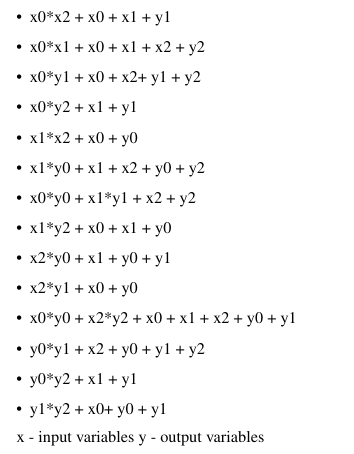
\includegraphics{pics/polynomials.png}
\end{figure}

\noindent\textbf{4.} Maximum degree of component function - 2\newline

\noindent\textbf{5.} Minimum degree of component function - 2\newline

\noindent\textbf{6.} Maximal differential probability - 0.25\newline

\noindent\textbf{7.} Absolute maximal linear bias - 2\newline

\noindent\textbf{8.} Relative maximal linear bias - 0.25\newline

\subsection{Cryptanalysis of PRINT Cipher}


While in related-key attacks on PRINTcipher-48/96 to find the weakness. On key-dependent permutation part related key have different values. By constructing related key of t-round the differential characteristics is of probability 2\textsuperscript{-t} so we will be able to extract the secret keys used PRINTcipher-48/96. 

To get back  80-bit secret key of PRINTcipher-48 it need 4 related key
PRINTcipher-48 need 2\textsuperscript{47} related-key chosen plaintexts with complexity of 2\textsuperscript{60.62}
To get back  160-bit secret key of PRINTcipher-96 it need 4 related key
PRINTcipher-96 need 2\textsuperscript{47} related-key chosen plaintexts with complexity of 2\textsuperscript{107}

\subsection{Construction of Related-Key Differential Characteristics on PRINTcipher}
Using attributes of a key-dependent permutation KP and S-box, steps to produce t round related-key differential characteristics on printcipher
\subsubsection{S-Box and Related-Key Properties on Key-Dependent Permutation :-}
 A key-dependent permutation KP\textsubscript{l} with a 3-bit input value (y0, y1, y2). Round-key of 2-bit is  is equal to (0,0) or  (0,1)

\begin{figure}[ht]
	\centering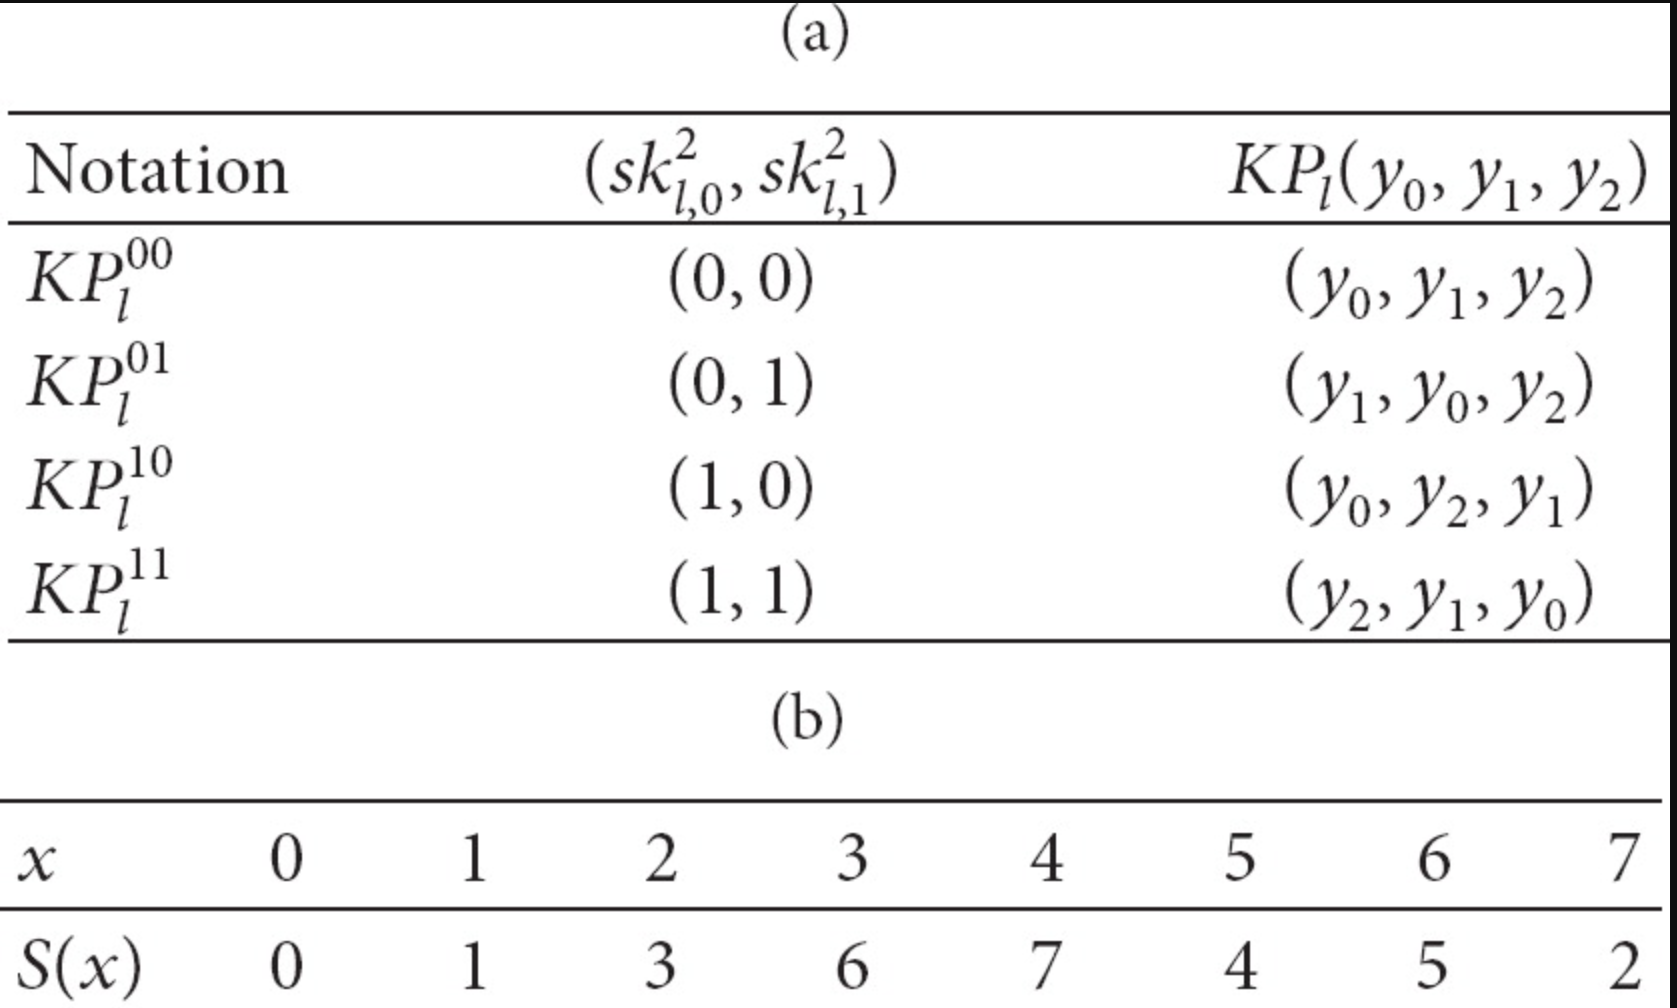
\includegraphics[width=5cm]{pics/3.png}
\end{figure}

\begin{figure}[ht]
	\centering
	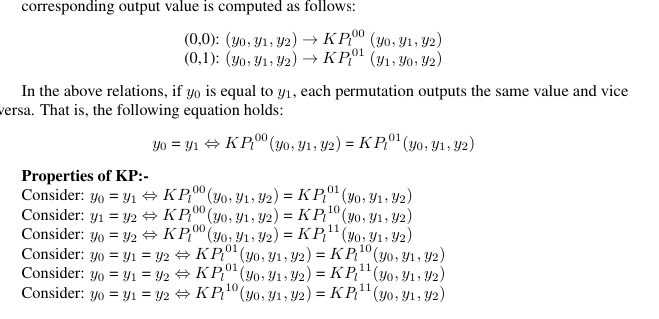
\includegraphics{pics/1.png}
\end{figure}

\subsubsection{PRINTcipher-48 Related-Key Differential Characteristics}

By evaluating similar key-pairs, we shall apply a few properties to the proposed attack.: \newline
\begin{figure}[ht]
	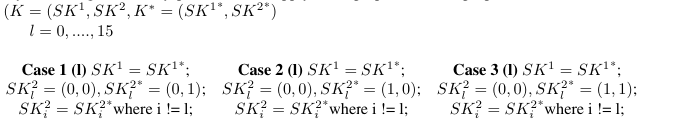
\includegraphics{pics/2.png}
\end{figure}


Suppose input difference of the target round is zero. If a paired key (k, k*) 
satisfies Case 1(0), key-dependent permutation incorporates a nonzero-related key difference. We will construct 1-round related-key differential characteristic 0 → Case1(0) with a probability of 2\textsuperscript{-1} under case 1. t-round related-key differential characteristic result further can be easily extended since PRINTcipher uses the identical round key for all round.

\begin{figure}[ht]
	\centering
	\includegraphics[height=8cm, width=12cm]{pics/oneround.png}
	\caption{One-round differential characteristic of related-key under Case-1-(0)}
\end{figure}


%\begin{figure}[h!]
	%\centering
	%\subfloat{ \includegraphics[height=5cm, width=7cm]{oneround.png}}
	%\caption{1-round related-key differential characteristic under Case 1 (0)}
%\end{figure}
\newpage
\subsubsection{PRINTcipher-48 Related-Key Cryptanalysis}
On PRINTcipher-48, a differential t-round related-key features with the probability of 2\textsuperscript{-t} can be built. Differential characteristics of related-key rely upon concrete key value. (K\textsubscript{0}\textsuperscript{0,0}, K\textsubscript{0}\textsuperscript{0,1}) and (K\textsubscript{0}\textsuperscript{1,0}, K\textsubscript{0}\textsuperscript{(1,1)}) key pairs are used to solve this issue.

\subsubsection{Basic Related-Key Attack on PRINTcipher-48}

Steps for attack procedure:-
\begin{itemize}
	\item Consider plain text strucutres of 4 plaintext each
	\item Wrong cipher text pair are deleted from the difference between ciphertexts.
	\item Output difference of round 45 should be 0 for a good ciphertext pair.
	\item Next, partial secret key is guessed.
\end{itemize}


\subsubsection{Complexities of Basic Related-Key Attack on PRINTcipher-48}
For plaintext strucutre step computational complexity is  \(2^{48}\) PRINTcipher-48 encryptions. Next, we discard wrong pair with ciphertext pairs servied is \(2^{10}(=8.2^{44}.2^{-37})\). Total computational complexity of the attack is \(2^{63}\).

\subsection{Experiment Results}
They needed to implement both PRINTcipher variations in VHDL and synthesise them using Synopsys DesignVision 2007.12 and the Virtual Silicon (VST) main cell library UMCL18G212T3, which is based on the UMC L180 0.18$\mu$m in order to calculate the effectiveness of the cipher. 1P6M logic process and has a typical voltage of 1.8 Volt
\begin{figure}[ht]
	\centering
	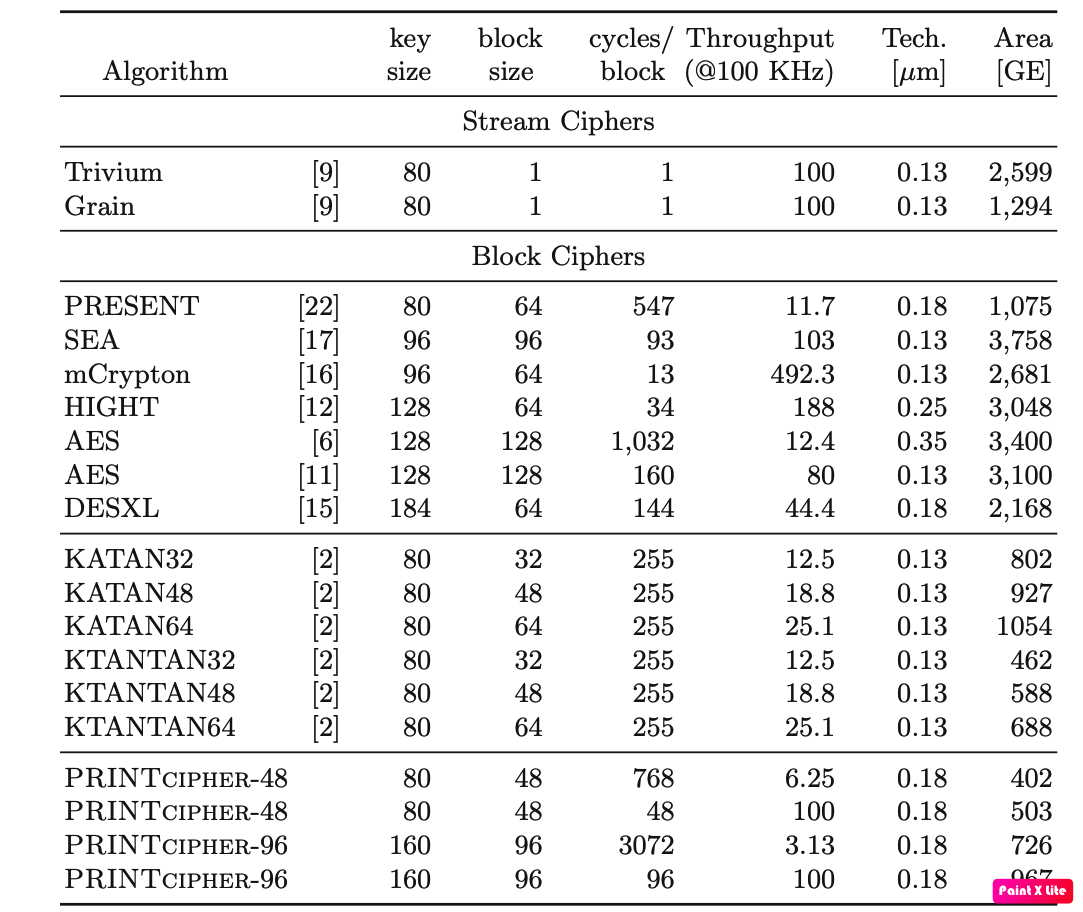
\includegraphics[height=7cm, width=12cm]{pics/hardware.png}
	\caption{comparison with some symmetric encryption algorithms.}
\end{figure}

\subsection{Conclusions}
In PRINTcipher they have considered the technology of IC-printing to see how it might influence the  cryptography that we use. They have proposed lightweight block cipher PRINTcipher that explicitly takes advantage of this new manufacturing approach. We related-key cryptanalysis of PRINTcipher. To recover the 80-bit secret key of PRINTcipher-48,related-key differential attack require \(2^{47}\) related-key chosen plaintexts with a computational complexity of \(2^{60.62}\). Further improvement can be done on the basic related-key attack on the full PRINTcipher-48 by considering 43-round instead of 48 round related-key.



\newpage
\subsection{Testvectors}
\begin{figure}[ht]
	\centering
	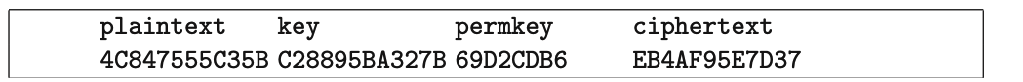
\includegraphics[height=1cm, width=5cm]{pics/testvector1.png}
	\caption{Sample Input and Output for PRINTcipher-48}
\end{figure}
\begin{figure}[ht]
	\centering
	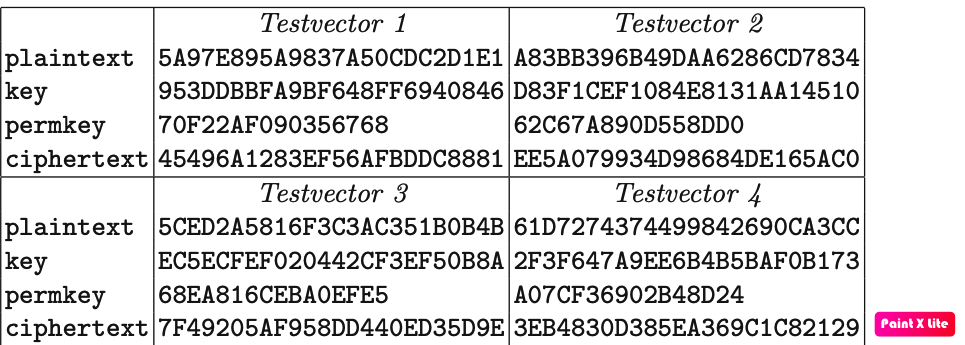
\includegraphics[height=3cm, width=7cm]{pics/testvector-2.png}
	\caption{Sample Testvectors for the cipher}
\end{figure}
\begin{figure}[ht]
	\centering
	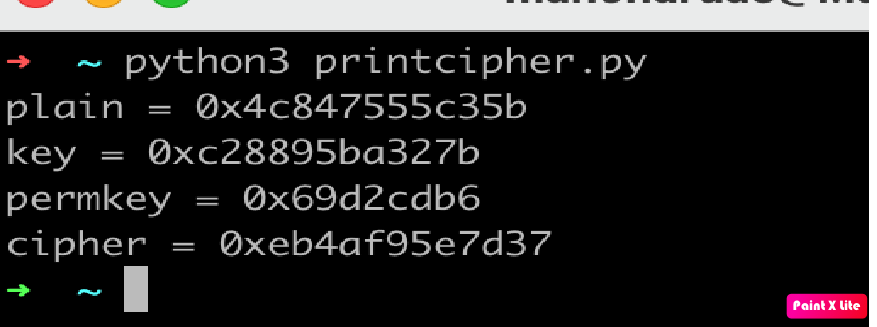
\includegraphics[height=6cm, width=10cm]{pics/pic_1.png}
	\caption{Sage implementation for Encryption of above plaintext}
\end{figure}
\begin{figure}[ht]
	\centering
	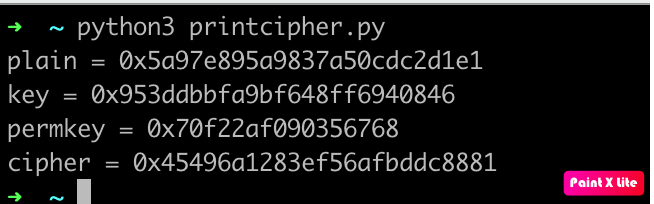
\includegraphics[height=6cm, width=10cm]{pics/pic_2.png}
	\caption{Sage implementation for Encryption of above plaintext}
\end{figure}
\begin{figure}[ht]
	\centering
	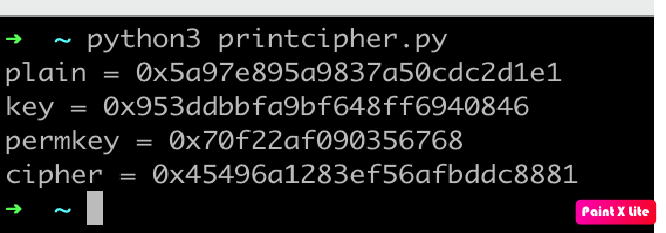
\includegraphics[height=6cm, width=10cm]{pics/pic_3.png}
	\caption{Sage implementation for Encryption of above plaintext}
\end{figure}


\newpage
\section{Code Snippet}
The code is implemented in Python.The code snippet is given below :-
\begin{figure}
	\centering
	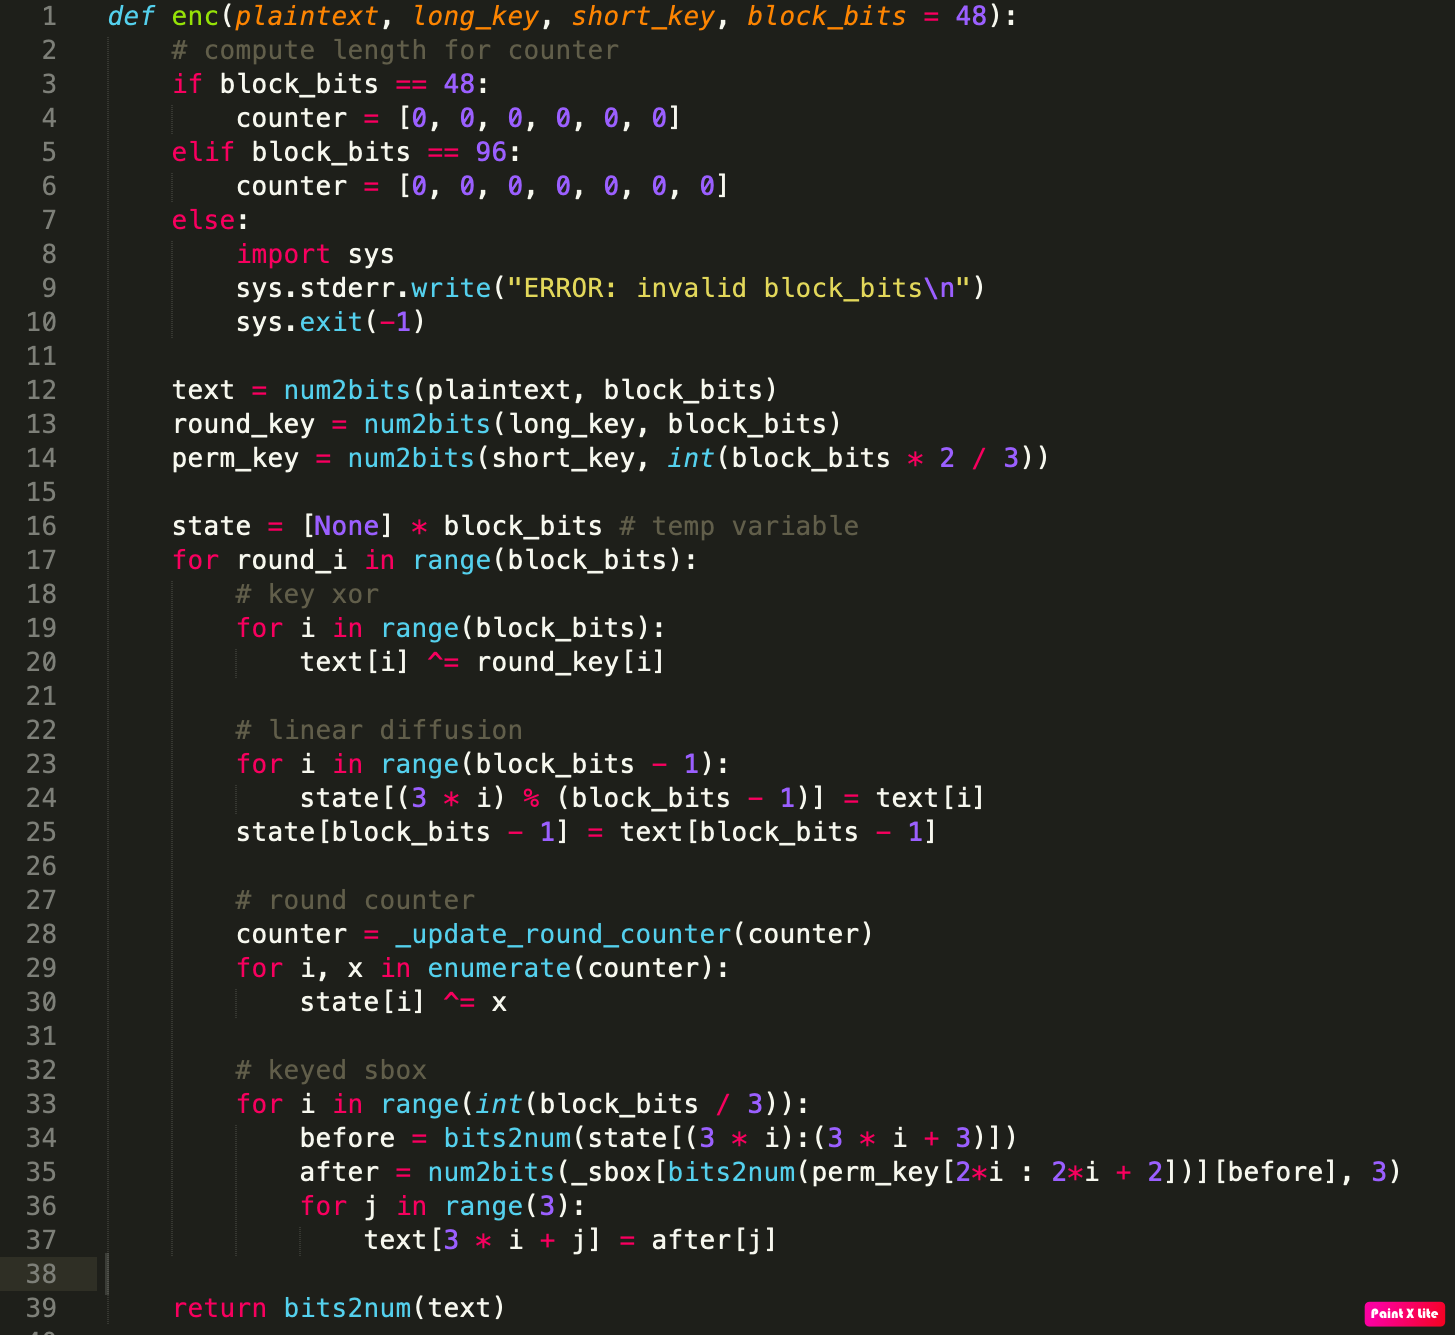
\includegraphics[height=10cm, width=\linewidth]{pics/codesnippet.png}
	\caption{Encryption function of PRINTcipher}
\end{figure}

\newpage
\subsection{Software Application Implementation}  
The motivation behind the development of the PRINT Cipher is the issue that in RFID applications, it is not required to change the key. It is rather considered as an overhead in RFID applications. Hence, PRINT Cipher is developed which requires a single key and it has been declared efficient for many applications such as fabrication of cheap RFID tags.The other concern was using a simple key schedule where subkeys are created in a simple fashion. So this cipher fulfilled the need and no working memory is needed for the subkey computations.

Here we are implementing an NFC/RFID compatible, platform independent login tool where the credentials are secured using PRINT Cipher. The usage of PRINT Cipher here provides fast access to RFID tags and NFC devices. The application provides a secure form of authentication that has been used in smart cards and mobile authentication. The basic idea is, that once you tap an authorized tag on the reader, the appropriate password is decrypted and typed on an emulated keyboard.
Once configured, you only need the HID driver on the host system. The basic idea is that when you tap a tag allowed by the reader, the corresponding password will be decrypted and entered into the emulated keyboard.
Here a simulator has been developed where a login form will be shown and the credentials entered will be encrypted and secured using PRINT Cipher and when they match a secured login is successfully done. Here to demonstrate the efficiency, PRINT Cipher-48 is used in the login tool.
As the cipher was designed by focusing more on the hardware efficiency, the performance of PRINT Cipher for any software implementation is slower [inefficient as compared to well known and widely used cipher like AES]than that of many well known and widely used ciphers like AES. It is observed that over a 64-bit platform, the performance of PRINT Cipher is 5-10 times slower than AES implementation.
\begin{figure}[ht]
	\centering
	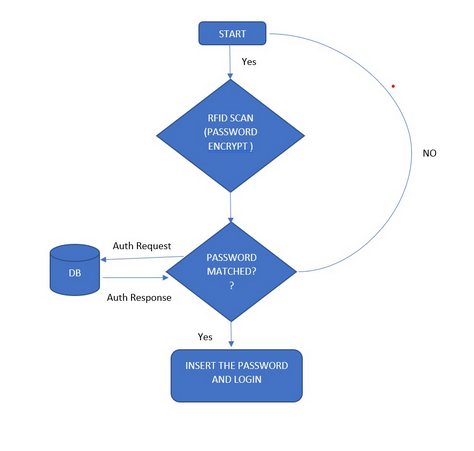
\includegraphics{pics/logintool.png}
	\caption{Figure: Login Mechanism Flow Chart}
\end{figure}

\section{References}

\begin{enumerate}[label={[\arabic*]}]
	
	\item Lars Knudsen, Gregor Leander, Axel Poschmann, and Matthew J.B. Robshaw, “PRINTcipher: A Block Cipher for IC-Printing”, CHES,  2010.
	
	\item Leander, Gregor and Abdelraheem, Mohamed Ahmed and AlKhzaimi, Hoda and Zenner, Erik, “A Cryptanalysis of PRINTcipher: The Invariant Subspace Attack”, Springer Berlin Heidelberg, 2011.
	
	\item Yuseop Lee, Kitae Jeong, Changhoon Lee, Jaechul Sung, Seokhie hong, “Related-key cryptanalysis on the full PRINTcipher suitable for IC-printing“, International Journal of Distributed Sensor Networks, 2014.
	
	\item Tadashi Okabe, “Efficient FPGA Implementations of PRINTCIPHER”, eISSN: 2349-5162, 2016.
	
	\item Daemen, Joan and Rijmen, Vincent, “The Block Cipher Rijndael”, Springer Berlin Heidelberg, 2000.
	
\end{enumerate}
%%%% 8. BILBIOGRAPHY %%%%
%\bibliographystyle{alpha}
%\bibliography{}
%%%% NOTES
% - Download abbrev3.bib and crypto.bib from https://cryptobib.di.ens.fr/
% - Use bilbio.bib for additional references not in the cryptobib database.
%   If possible, take them from DBLP.

\end{document}
